% --- ETUDE DE CAS ---
\section*{Étude de cas: La rançon du Cyberespace}
\addcontentsline{toc}{section}{Étude de cas: La rançon du Cyberespace}

\section*{AAV}
\addcontentsline{toc}{section}{AAV}
\begin{itemize}
  \item [5] Renforcer la vision globale du Système d'Information
  \item [3] Inventorier les différents composants du Système d'Information
  \item [4] Etablir une cartographie du Système d'Information
  \item [4] Analyser de manière holistique la sécurité du S.I.
  \item [1] Rappeler le cadre légal
  \item [3] Préparer des scripts sous Linux
  \item [5] Réorganiser la sécurité d'une infrastructure
\end{itemize}

\subsection*{Mots clés}
\phantomsection
\addcontentsline{toc}{subsection}{Mots clés}
\begin{itemize}
  \item Ransomware
  \item Système d'information
  \item ANSSI
  \item MOOC
  \item ERP
  \item CTO
  \item DSI
  \item CNIL
  \item Vecteur d'attaque
  \item Cybermenaces
  \item Durcissement
  \item Anti Virus
  \item Privilèges
  \item RSSI
  \item Infection par PDF
  \item RGPD
\end{itemize}

\subsection*{Contexte}
\phantomsection
\addcontentsline{toc}{subsection}{Contexte}
Léo arrive dans un climat tendu suite à une attaque par ransomware sur une entreprise voisine. Sa responsable saisie cette opportunité pour renforcer la sécurité et sensibiliser le personnel de BERRIA.

\subsection*{Problématique}
\phantomsection
\addcontentsline{toc}{subsection}{Problématique}
Comment sécuriser le système d'information de BERRIA contre les ransomwares et autres cybermenaces, tout en sensibilisant efficacement le personnel aux bonnes pratiques de sécurité informatique?

\subsection*{Contraintes}
\phantomsection
\addcontentsline{toc}{subsection}{Contraintes}
\begin{itemize}
  \item Windows
  \item ANSSI
  \item MOOC
  \item Wifi Invité
  \item Cadre légale
\end{itemize}

\subsection*{Généralisation}
\phantomsection
\addcontentsline{toc}{subsection}{Généralisation}
\begin{itemize}
  \item Cybersécurité
  \item Sensibilisation
  \item Administration Système
  \item Législation (RGPD)
\end{itemize}

\subsection*{Livrables}
\phantomsection
\addcontentsline{toc}{subsection}{Livrables}
\begin{itemize}
  \item Plaquette de prévention
  \item Script de Sécurisation W10
  \item Rapport d'étude
\end{itemize}

\subsection*{Pistes de solutions}
\phantomsection
\addcontentsline{toc}{subsection}{Pistes de solutions}
\begin{itemize}
  \item MOOC SecNum Académie
  \item Guide ANSSI
  \item Principe de moindre privilège
  \item Kiosk Mode
  \item Analyse des vecteurs d'attaque
  \item Sauvegarde déconnectée
\end{itemize}

\subsection*{Plan d'action}
\phantomsection
\addcontentsline{toc}{subsection}{Plan d'action}
\begin{itemize}
  \item Définir les mots clés
  \item Etudier les ressources
  \item Etudier les différentes cybermenaces et vecteurs d'attaques
  \item Comprendre la différence entre SI et SI informatique
  \item Suivre MOOC de l'ANSSI
  \item Recenser les régles de la CNIL
  \item Rechercher les méthodes de durcissement Windows 10
  \item Mettre en place une maquette pour tester la configuration
  \item Rédiger la plaquette de sensibilisation
  \item Rédiger le rapport final
\end{itemize}

\clearpage
\section*{Démarche~: La rançon du Cyberespace}
\addcontentsline{toc}{section}{Démarche~: La rançon du Cyberespace}

\subsection*{Définition: Mots clés}
\phantomsection
\addcontentsline{toc}{subsection}{Définition: Mots clés}

\noindent \textbf{Ransomware}:
Un ransomware est un logiciel malveillant qui chiffre ou exfiltre des données et peut bloquer l'accès aux systèmes jusqu'au paiement d'une rançon.

\begin{center}
  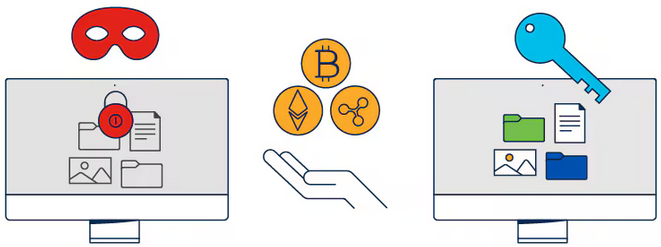
\includegraphics[width=0.5\textwidth]{contents/img/ransomware.png}
\end{center}

Les vecteurs d'infection les plus courants sont :
\begin{itemize}
    \item le phishing (pièces jointes ou liens malveillants) ;
    \item les services exposés non protégés (RDP, SMB) ;
    \item les vulnérabilités non corrigées ;
    \item la compromission de comptes à privilèges.
\end{itemize}

Mesures essentielles de prévention et réponse :
\begin{itemize}
    \item sauvegardes régulières, testées et idéalement isolées (\textit{air-gapped}) ;
    \item segmentation réseau ;
    \item authentification multi-facteur (MFA) ;
    \item gestion stricte des privilèges ;
    \item détection comportementale (EDR) ;
    \item plan de réponse à incident incluant préservation des preuves et notification des autorités (ANSSI / CERT-FR).
\end{itemize}
Le paiement d'une rançon est déconseillé : aucune garantie de récupération et encourage la criminalité. Il est recommandé d'impliquer les forces de l'ordre et les CERT nationaux.

\newpage

\noindent \textbf{Système d'information (SI)}:
Un SI regroupe l'ensemble des ressources techniques, humaines et organisationnelles permettant de collecter, traiter, stocker et diffuser l'information.
Un SI maîtrisé repose sur :
\begin{itemize}
    \item une cartographie des actifs (postes, serveurs, applications, données) ;
    \item une gestion rigoureuse des identités et des accès (IAM) ;
    \item un pilotage clair (rôles, responsabilités, procédures) ;
    \item des sauvegardes fiables et testées ;
    \item une supervision continue et une gestion d'incidents structurée ;
    \item un inventaire centralisé (CMDB).
\end{itemize}

\vspace{0.5cm}

\noindent\textbf{ANSSI} :  
L'Agence Nationale de la Sécurité des Systèmes d'Information est l'autorité française en cybersécurité.

\begin{wrapfigure}{r}{0.2\textwidth}
    \vspace{-25pt}
    \begin{center}
        
\includegraphics[width=0.15\textwidth]{contents/img/ANSSI.png}
    \end{center}
\end{wrapfigure}

Ses rôles principaux :
\begin{itemize}
    \item publication de guides et bonnes pratiques ;
    \item coordination d'incidents majeurs via le CERT-FR ;
    \item qualification d'acteurs et solutions ;
    \item sensibilisation et accompagnement.
\end{itemize}

\vspace{0.5cm}

\noindent \textbf{MOOC}:
Formations en ligne ouvertes permettant de monter en compétences en sécurité.  
Privilégier les MOOC de l'ANSSI, d'universités ou de fournisseurs reconnus, avec exercices pratiques.

\vspace{0.5cm}

\noindent \textbf{ERP}:
Un ERP centralise des processus métiers critiques (RH, finances, achats, production).  
Mesures de sécurité essentielles :
\begin{itemize}
    \item contrôle strict des accès (IAM, MFA) ;
    \item gestion des correctifs ;
    \item segmentation réseau ;
    \item chiffrement des données ;
    \item sauvegardes applicatives cohérentes.
\end{itemize}

\vspace{0.5cm}

\noindent \textbf{CTO}:
Le Chief Technology Officer définit la stratégie technologique.  
Rôles liés à la sécurité :
\begin{itemize}
    \item intégrer le \textit{security by design} dans l'architecture ;
    \item arbitrer les investissements (EDR, SIEM, backups) ;
    \item aligner vision technologique et contraintes de risque.
\end{itemize}

\vspace{0.5cm}

\noindent \textbf{DSI}:
Le Directeur des Systèmes d'Information gère l'exploitation du SI.  
Responsabilités clés :
\begin{itemize}
    \item mise en œuvre de la politique de sécurité ;
    \item mises à jour, sauvegardes, supervision ;
    \item gestion des incidents ;
    \item conformité réglementaire (RGPD).
\end{itemize}

\noindent \textbf{CNIL} :  
La Commission Nationale de l'Informatique et des Libertés (CNIL) est l'autorité française chargée de veiller au respect de la protection des données personnelles (RGPD). En cas d'incident de sécurité impliquant des données personnelles, obligations et bonnes pratiques :
\begin{itemize}
  \item documenter immédiatement l'incident (nature, périmètre, causes, données concernées) ;
  \item évaluer l'impact et le risque pour les personnes concernées (DPIA si nécessaire) ;
  \item notifier la CNIL dans les 72 heures lorsqu'un risque pour les droits et libertés est probable ;
  \item informer les personnes concernées si le risque est élevé, en précisant les mesures d'atténuation recommandées ;
  \item consigner l'incident et les actions correctives dans le registre des violations ;
  \item coopérer avec la CNIL et le Délégué à la Protection des Données (DPO) durant l'enquête ;
  \item mettre en place des mesures préventives : minimisation des données, chiffrement, contrôle d'accès, sauvegardes isolées, journalisation et sensibilisation du personnel.
\end{itemize}
Sanctions possibles : mesures correctrices et amendes administratives prévues par le RGPD en cas de manquement grave.

\noindent \textbf{RGPD} :  
Le Règlement Général sur la Protection des Données (RGPD) encadre le traitement des données à caractère personnel au sein de l'Union européenne. Il garantit la protection des droits et libertés des personnes physiques et impose des obligations aux organisations qui collectent, traitent ou conservent ces données.

Principes clés :
\begin{itemize}
  \item licéité, loyauté et transparence ;
  \item limitation des finalités ;
  \item minimisation des données ;
  \item exactitude et conservation limitée ;
  \item intégrité et confidentialité (sécurité des traitements).
\end{itemize}

\newpage

Obligations principales :
\begin{itemize}
  \item disposer d'une base légale pour chaque traitement (consentement, exécution de contrat, obligation légale, intérêt légitime, etc.) ;
  \item respecter et faciliter l'exercice des droits des personnes (accès, rectification, effacement, limitation, portabilité, opposition) ;
  \item mettre en place des mesures techniques et organisationnelles adaptées (pseudonymisation, chiffrement, contrôle d'accès, journalisation) ;
  \item documenter les traitements et tenir un registre des activités lorsque requis ;
  \item notifier les violations de données à l'autorité de contrôle compétente dans les 72 heures et informer les personnes concernées si le risque est élevé ;
  \item désigner un délégué à la protection des données (DPO) lorsque nécessaire et encadrer les transferts hors UE.
\end{itemize}

\noindent Sanctions : la non‑conformité peut entraîner des mesures correctrices et des amendes administratives importantes (jusqu'à 20 millions d'euros ou 4\% du chiffre d'affaires mondial annuel).

\vspace{0.5cm}

\noindent \textbf{Vecteurs d'attaque}:
Méthodes utilisées par un attaquant pour compromettre un système :

\begin{center}
        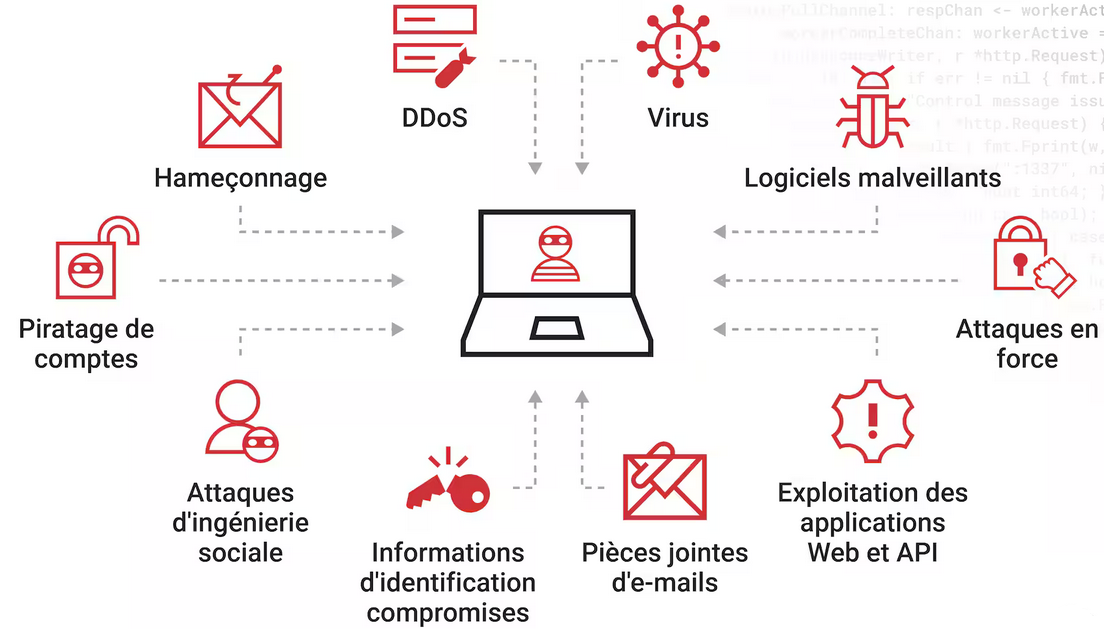
\includegraphics[width=0.8\textwidth]{contents/img/vecteurattaque.png}
\end{center}

\begin{itemize}
    \item phishing / spear-phishing ;
    \item pièces jointes malveillantes ;
    \item vulnérabilités non corrigées ;
    \item services exposés sans durcissement ;
    \item compromission de la chaîne d'approvisionnement ;
    \item abus de comptes tiers.
\end{itemize}

\newpage

\noindent \textbf{Cybermenaces}:
Regroupe malwares, ransomware, DDoS, espionnage, vol d'identifiants, menaces internes.  
Une stratégie efficace repose sur :
\begin{itemize}
    \item threat modelling ;
    \item indicateurs de compromission (IOC) ;
    \item threat intelligence ;
    \item corrélation d'événements via SIEM.
\end{itemize}

\vspace{0.5cm}

\noindent \textbf{Durcissement}:
Réduction de la surface d'attaque :
\begin{itemize}
    \item suppression des services inutiles ;
    \item application des correctifs ;
    \item moindre privilège ;
    \item MFA, politiques robustes ;
    \item protections natives (pare-feu, AppLocker, ASR) ;
    \item configuration as code.
\end{itemize}

\vspace{0.5cm}

\noindent \textbf{Antivirus}:
Un antivirus (AV) détecte et bloque principalement les menaces connues via des signatures et des heuristiques, mais il ne suffit pas à lui seul face aux attaques ciblées et aux menaces sans signature. \\
Pour une protection robuste, on recommande de :
\begin{itemize}
  \item coupler l'AV avec une solution EDR pour la détection comportementale, l'investigation et la réponse automatisée ;
  \item maintenir à jour les signatures, le moteur et le système d'exploitation, et activer les protections cloud/heuristiques ;
  \item centraliser les alertes et corréler les événements dans un SIEM pour détecter les campagnes et les mouvements latéraux ;
  \item définir des politiques d'exclusion maîtrisées et des procédures d'isolement pour limiter l'impact des faux positifs ;
  \item compléter par segmentation réseau, sauvegardes isolées, MFA, contrôles d'accès stricts et sensibilisation des utilisateurs.
\end{itemize}

\vspace{0.5cm}

\noindent \textbf{Privilèges}:
Gestion conforme au principe du moindre privilège :
\begin{itemize}
    \item séparation comptes admin / utilisateurs ;
    \item élévation temporaire (\textit{just-in-time}) ;
    \item revue régulière des droits ;
    \item MFA obligatoire ;
    \item journalisation renforcée.
\end{itemize}

\vspace{0.5cm}

\noindent \textbf{RSSI}:
Le Responsable de la Sécurité des Systèmes d'Information pilote la stratégie de sécurité.
Rôles clés :
\begin{itemize}
    \item évaluation des risques ;
    \item définition de la politique de sécurité ;
    \item sensibilisation et formation ;
    \item gestion des incidents ;
    \item conformité réglementaire.
    \item supervision des outils de sécurité.
\end{itemize}

\vspace{0.5cm}

\noindent \textbf{Infections via PDF}:
Les PDF peuvent embarquer scripts ou objets malveillants.  
Mesures :
\begin{itemize}
    \item désactivation de JavaScript dans les lecteurs ;
    \item mises à jour régulières ;
    \item filtrage et sandbox des pièces jointes ;
    \item conversion en texte pour analyse ;
    \item sensibilisation des utilisateurs.
\end{itemize}

\newpage

\section*{Corbeille d'Excercice}
\addcontentsline{toc}{section}{Corbeille d'Excercice}

\subsection*{Introduction à la sécurisation du poste de travail et à PowerShell}
\phantomsection
\addcontentsline{toc}{subsection}{Introduction à la sécurisation du poste de travail et à PowerShell}

\noindent \textbf{Introduction}: 
PowerShell se présente sous deux formes :
\begin{itemize}
  \item La console PowerShell (PS) qui interprète les commandes en ligne (Figure à gauche),
  \item Un environnement graphique de développement de scripts – PowerShell Integrated Scripting Environment (PS-ISE) (figure à droite).
\end{itemize}

\vspace{0.5cm}

\begin{figure}[h!]
    \centering
    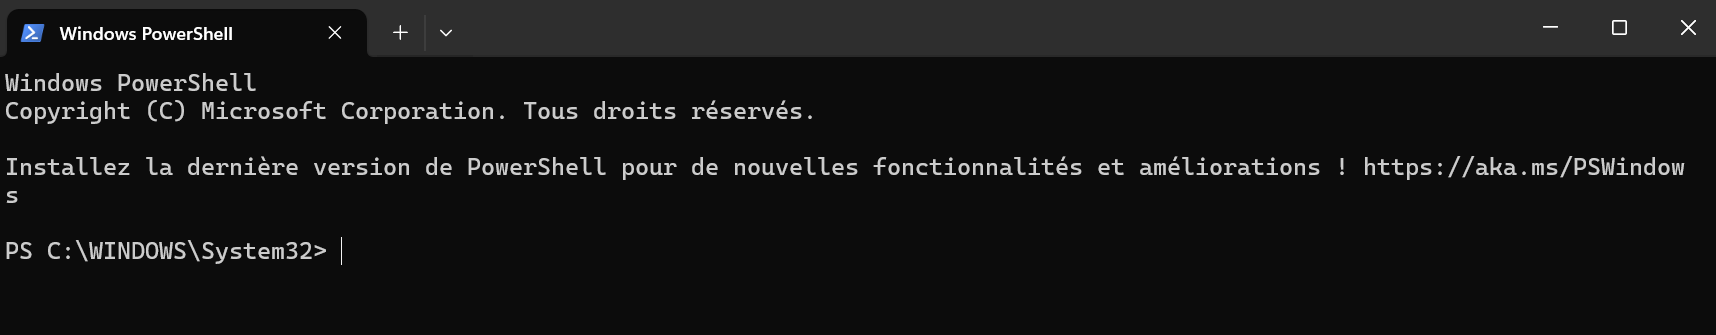
\includegraphics[width=0.4\textwidth]{contents/img/powershell_ps.png}
    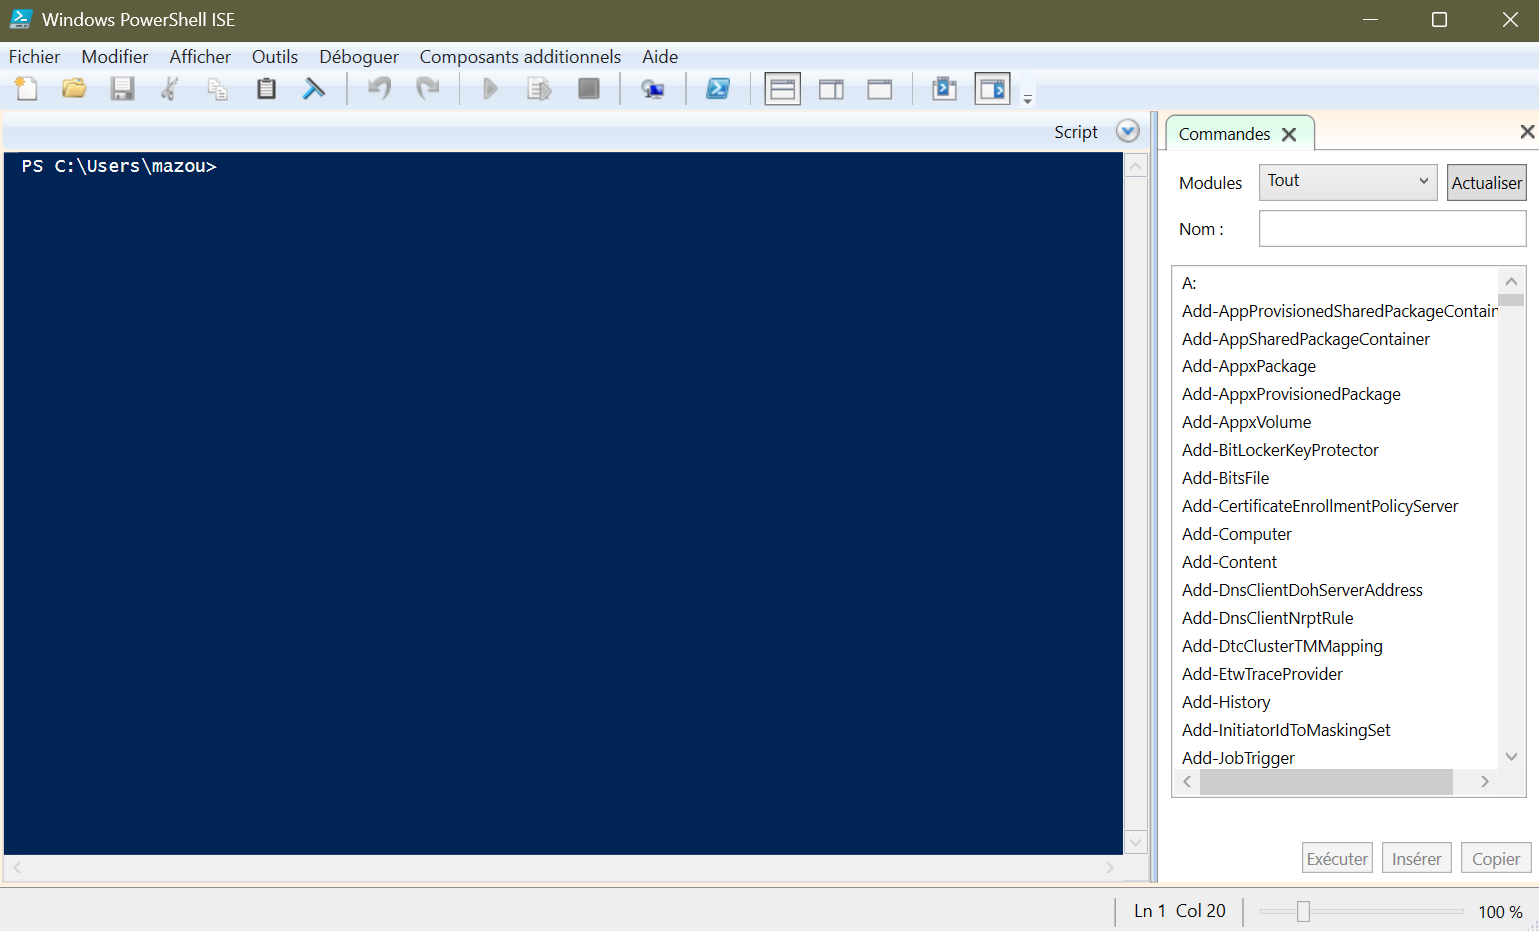
\includegraphics[width=0.4\textwidth]{contents/img/powershell_ise.png}
    \caption{Console PowerShell et PowerShell ISE}
\end{figure}

\noindent Pour lancer PS, aller dans le menu \textbf{Démarrer > Tous les Programmes > Accessoires > WindowsPowerShell} et choisissez l'interface souhaitée, Il est également possible de lancer PS avec l'interpréteur classique de commandes de Windows (cmd.exe) avec la commande \textbf{PowerShell}.

\noindent Les “cmdlet” sont composées d'une paire de la forme “verbe” -“nom” destinées à en faciliter la
mémorisation.

\begin{center}
  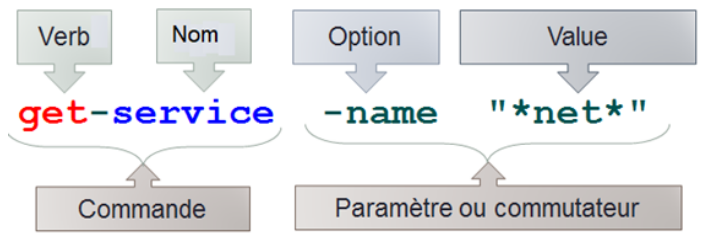
\includegraphics[width=0.4\textwidth]{contents/img/cmdlet.png}
\end{center}

\noindent \textbf{Exemples de cmdlet} :
\begin{itemize}
  \item Get-Process : Affiche la liste des processus en cours d'exécution.
  \item Get-Service : Affiche la liste des services installés sur le système.
  \item Get-EventLog : Affiche les journaux d'événements du système.
  \item Set-ExecutionPolicy : Modifie la politique d'exécution des scripts PowerShell.
\end{itemize}

\newpage

\noindent PowerShell propose 4 modes d'exécution des scripts :
\begin{itemize}
  \item Restricted : Mode par défaut, n'autorise pas l'exécution de scripts.
  \item AllSigned : N'autorise l'exécution que des scripts signés par un éditeur de confiance.
  \item RemoteSigned : Autorise l'exécution des scripts locaux non signés, mais exige que les scripts téléchargés soient signés.
  \item Unrestricted : Autorise l'exécution de tous les scripts, mais affiche un avertissement pour les scripts téléchargés.
\end{itemize}

\vspace{0.5cm}

\noindent En tant que script PowerShell permet de déclarer une variable.
\begin{itemize}
  \item \textbf{Nom / Identifiant} : Étiquette permettant de référencer la variable dans le code.
  \item \textbf{Type} : Définit le format des données (entier, flottant, chaîne, objet) et les opérations possibles.
  \item \textbf{Valeur} : Contenu actuel stocké dans la variable.
  \item \textbf{Portée (scope)} : Zone du programme où la variable est accessible (locale, globale, de bloc, de fonction).
  \item \textbf{Durée de vie (lifetime)} : Période pendant laquelle la variable existe en mémoire (statique, automatique, dynamique).
  \item \textbf{Mutabilité / Constante} : Indique si la valeur peut être modifiée après initialisation.
  \item \textbf{Allocation mémoire / Taille} : Emplacement et taille en mémoire (pile, tas, adresse) et contraintes associées.
\end{itemize}

\vspace{0.5cm}

\noindent \textbf{Exemple de script opérationnels} :

1. Inviter l'utilisateur à saisir son prénom et son âge, et afficher une phrase récapitulative « Bonjour XXX
vous avez Y ans. »

\begin{verbatim}
$prenom = Read-Host "Entrez votre prénom"
$age = Read-Host "Entrez votre âge"
Write-Host "Bonjour $prenom, vous avez $age ans."
\end{verbatim}


2. Voici un jeu.
Vous devez inviter l'utilisateur à deviner un nombre :
\begin{itemize}
  \item Tirer un nombre aléatoire entier entre 0 et 100
  \item Inviter l'utilisateur à entrer son essai
  \begin{itemize}
    \item Si l'utilisateur est plus haut, afficher en rouge « Trop haut ! mon nombre est plus bas. »
    \item Si l'utilisateur est plus bas, afficher en gris « Trop bas ! mon nombre est supérieur. »
    \item Si l'utilisateur devine le nombre, afficher en vert « bravo, vous avez trouvé en XXX essais ! » (et compter le nb d'essais)
  \end{itemize}
\end{itemize}

\begin{center}
  \begin{verbatim}
  $nombreSecret = Get-Random -Minimum 0 -Maximum 100
  $essais = 0
  do {
    $essais++
    $essai = Read-Host "Devinez le nombre (entre 0 et 100)"
    if ($essai -lt $nombreSecret) {
      Write-Host "Trop bas ! mon nombre est supérieur."
      -ForegroundColor Gray
    }
    elseif ($essai -gt $nombreSecret) {
      Write-Host "Trop haut ! mon nombre est plus bas."
      -ForegroundColor Red
    }
  } while ($essai -ne $nombreSecret)
  Write-Host "Bravo, vous avez trouvé en $essais essais !"
  -ForegroundColor Green
  \end{verbatim}
\end{center}


\vspace{0.5cm}

3. Comment lancer Notepad (ou un autre programme...) s'il n'est pas déjà lancé en mémoire ?

\begin{center}
  \begin{verbatim}
  $processName = "notepad"
  $process = Get-Process -Name $processName -ErrorAction SilentlyContinue
  if ($null -eq $process) {
      Start-Process $processName
      Write-Host "$processName a été lancé."
  } else {
      Write-Host "$processName est déjà en cours d'exécution."
  }
  \end{verbatim}
\end{center}

\vspace{0.5cm}

\subsection*{Gérer les utilisateur locaux sur un poste avec un système Windows}
\phantomsection
\addcontentsline{toc}{subsection}{Gérer les utilisateur locaux sur un poste avec un système Windows}

\noindent Lorsqu'ils sont mal utilisés, les privilèges d'administrateur local d'un PC Windows peuvent causer de graves dommages à l'ordinateur de l'utilisateur, exposer d'autres ordinateurs sur un réseau donné et rendre les machines plus vulnérables aux virus et aux acteurs malveillants, ce qui crée encore plus de défis et de problèmes pour le service informatique de l'organisation.

\noindent Windows permet d’ajouter plusieurs comptes d’utilisateur pour utiliser le même appareil, ce qui permet à chaque utilisateur d’avoir ses propres paramètres, documents et applications. 

\newpage

\noindent Les comptes d’utilisateur locaux sont définis localement sur un appareil et peuvent se voir attribuer des droits et des autorisations uniquement sur l’appareil. Les comptes d’utilisateur locaux sont utilisés pour sécuriser et gérer l’accès aux ressources sur un appareil, pour les services ou les utilisateurs.

\begin{itemize}
  \item \textbf{Les comptes d’utilisateur locaux par défaut} sont des comptes intégrés qui sont créés automatiquement lorsque le système d’exploitation est installé. Les comptes d’utilisateur locaux par défaut ne peuvent pas être supprimés ou supprimés et ne fournissent pas l’accès aux ressources réseau.
  \item \textbf{Le compte d’administrateur local par défaut} est un compte d’utilisateur pour l’administration du système. Le compte Administrateur est le premier compte créé pendant l’installation de Windows. Le compte administrateur par défaut ne peut pas être supprimé ou verrouillé, mais il peut être renommé ou désactivé.
  \item \textbf{Le compte Invité} permet aux utilisateurs occasionnels ou ponctuels, qui n’ont pas de compte sur l’ordinateur, de se connecter temporairement au serveur local ou à l’ordinateur client avec des droits d’utilisateur limités. Par défaut, le compte Invité est désactivé et a un mot de passe vide02
\end{itemize}

\vspace{0.5cm}

\noindent \textbf{Exemple de script pour gérer les utilisateurs locaux} :

4. Comment créer un compte utilisateur local dans Windows 10 ou 11 ?

\begin{center}
  \begin{verbatim}
    $username = "NouvelUtilisateur"
    $password = "MotDePasseSecurise123!" |
      ConvertTo-SecureString -AsPlainText -Force
    New-LocalUser -Name $username 
      -Password $password 
      -FullName "Utilisateur Local" 
      -Description "Compte utilisateur local créé via PowerShell"
    Add-LocalGroupMember -Group "Users" -Member $username
    Write-Host "Le compte utilisateur local '$username' a été créé 
    avec succès."
  \end{verbatim}
\end{center}

5. Comment accéder à la base de compte locale sur un PC Windows 10 ou 11 avec un outil graphique? (sauf pour l'édition Famille)

\begin{center}
  \begin{verbatim}
    lusrmgr.msc
  \end{verbatim}
\end{center}

6. Où se trouve la base des comptes locaux dans le système de fichier d'un poste Windows ?

\begin{center}
  \begin{verbatim}
    C:\Windows\System32\config\SAM
  \end{verbatim}
\end{center}

\newpage

7. Comment utiliser PowerShell pour réaliser les actions suivantes ?
\begin{itemize}
  \item Listez les comptes utilisateurs locaux de la machine.
  \item Créez un nouveau compte non administrateur.
  \item Créez un nouveau compte administrateur.
\end{itemize}

\noindent Attention, dans les 2 cas il faut demander de taper le login souhaité, le mot de passe et re-taper le mot de passe pour vérification

\begin{center}
  \begin{verbatim}
    # Lister les comptes utilisateurs locaux
    Get-LocalUser

    # Créer un nouveau compte non administrateur
    $username = Read-Host "Entrez le nom d'utilisateur"
    $password = Read-Host "Entrez le mot de passe" -AsSecureString
    New-LocalUser -Name $username 
      -Password $password 
      -FullName "Utilisateur Local" 
      -Description "Compte utilisateur local non administrateur"
    Add-LocalGroupMember -Group "Users" -Member $username
    Write-Host "Le compte utilisateur local '$username' a été créé 
    avec succès."

    # Créer un nouveau compte administrateur
    $adminUsername = Read-Host "Entrez le nom d'utilisateur
    administrateur"
    $adminPassword = Read-Host "Entrez le mot de passe 
    administrateur" -AsSecureString
    New-LocalUser -Name $adminUsername 
      -Password $adminPassword 
      -FullName "Administrateur Local" 
      -Description "Compte administrateur local"
    Add-LocalGroupMember -Group "Administrators" -Member $adminUsername
    Write-Host "Le compte administrateur local '$adminUsername' a 
    été créé avec succès."
  \end{verbatim}
\end{center}

\newpage

\subsection*{La sécurité des postes Windows avec Windows Security}
\phantomsection
\addcontentsline{toc}{subsection}{La sécurité des postes Windows avec Windows Security}

\noindent L'application de sécurité Windows (Windows Security) existe sur les postes Windows et les serveurs Windows. L'interface graphique est disponible sur Windows 10 et 11. Les fonctions peuvent être gérées en PowerShell.

% Remarque : ce tableau utilise des couleurs (requiert \usepackage[table]{xcolor} dans le préambule)
\begingroup
\definecolor{headercolor}{HTML}{DCE6F1}    % couleur ligne d'entête
\definecolor{firstcol}{HTML}{F2F8FF}       % couleur première colonne
\setlength{\extrarowheight}{3pt}
\begin{table}[h!]
  \centering
  \label{tab:securite}
  \small
  \begin{tabular}{>{\columncolor{firstcol}}p{4cm} p{5cm} p{5cm}}
    \rowcolor{headercolor}
    \textbf{Fonctionnalité} & \textbf{Windows 10 Éducation} & \textbf{Windows Server 2022 Standard} \\
    \hline
    Application "Sécurité Windows" (GUI) & Complète et activée par défaut & Présente mais souvent désactivée ou minimale \\
    Microsoft Defender Antivirus & Activé et fonctionnel par défaut & Inclus, mais peut être désactivé \\
    Protection en temps réel & Activée & Désactivée par défaut \\
    Protection basée sur le cloud & Activée & Désactivée par défaut, à activer \\
    Mises à jour de signatures Defender & Automatiques via Windows Update & Automatiques si Defender est actif \\
    Protection contre les ransomwares & Disponible avec "Accès contrôlé aux dossiers" & Fonction disponible mais désactivée par défaut \\
    Pare-feu Windows Defender & Activé, configurable via GUI & Activé par défaut \\
    Sécurité matérielle (TPM, Secure Boot) & Compatible, dépend du matériel & Compatible, dépend du serveur \\
    Notifications de sécurité & Activées & Désactivées dans de nombreux cas (serveur) \\
    Gestion via GPO & Oui, pour toutes les fonctionnalités & Oui, fortement recommandée \\
    Gestion via PowerShell (Get-Mp*) & Oui & Oui \\
    Microsoft Defender SmartScreen & Activé & Non présent ou inactif sur les serveurs \\
    Contrôle des applications (AppLocker) & Oui (via GPO) & Oui (via GPO, souvent utilisé) \\
    Mode multi-utilisateurs / domaine & Compatible avec AD, mais usages "poste client" & Conçu pour les domaines et serveurs \\
  \end{tabular}
  \caption{Tableau récapitulatif des mesures de sécurisation}
\end{table}
\endgroup

\newpage

\subsection*{Protection Antivirus}
\phantomsection
\addcontentsline{toc}{subsection}{Protection Antivirus}
\noindent Pour tester le fonctionnement d’un antivirus nous utiliser le fichier de test Eicar, qui est une chaîne de caractères, écrite dans un fichier informatique.

\noindent Créez un fichier texte (utilisez le Bloc-notes de Windows par exemple) avec le contenu suivant que vous pouvez copier et coller dans votre fichier :
\begin{center}
  \begin{verbatim}
    X5O!P%@AP[4\PZX54(P^)7CC)7}$EICAR-STANDARD-ANTIVIRUS-TEST-FILE!$H+H*
  \end{verbatim}
\end{center}

\noindent Renommez ensuite le fichier créé pour en changer l’extension de « .txt » en « .com ».

\vspace{0.5cm}

8. Que se passe-t-il ? Expliquez pourquoi.

\begin{verbatim}
# Lorsque le fichier Eicar est créé avec l'extension .com,
# l'antivirus Windows Defender le détecte immédiatement
# comme une menace potentielle et le met en quarantaine ou le supprime.
# Cela se produit parce que le contenu du fichier correspond à la
# signature de test standard utilisée pour vérifier le bon fonctionnement
# des logiciels antivirus.
\end{verbatim}

\vspace{0.5cm}

9. Quelle est la commande PowerShell qui installe la fonctionnalité Antivirus Microsoft Defender sur un serveur Windows 2022 ? et celle que l’on peut utiliser pour vérifier que le service fonctionne ?

\begin{verbatim}
# Pour installer Microsoft Defender Antivirus sur Windows Server 2022
Install-WindowsFeature -Name Windows-Defender-Features

# Pour vérifier que le service fonctionne
Get-Service -Name WinDefend
\end{verbatim}

\vspace{0.5cm}

10. Est-ce que la sécurité Windows propose des fonctions pour traiter les ransomware ?

\begin{verbatim}
# Oui, Windows Security propose une fonctionnalité appelée
# "Accès contrôlé aux dossiers" qui protège les dossiers
# contre les modifications non autorisées, y compris celles
# effectuées par des ransomwares.
\end{verbatim}

\subsection*{Mise à jour des systèmes d'exploitation}
\phantomsection
\addcontentsline{toc}{subsection}{Mise à jour des systèmes d'exploitation}

\noindent Avoir des systèmes d'exploitations à jour est très important pour sécuriser un système informatique. Lorsqu’un ordinateur est à jour, c’est-à-dire que toutes les mises à jour publiées par l’éditeur, en l’occurrence ici Microsoft, sont installées, il est protégé contre les vulnérabilités connues. 

\noindent A contrario, les ordinateurs où les mises à jour ne sont pas installées sont vulnérables : un logiciel malveillant peut en tirer profit pour compromettre cet ordinateur. Ceci est bien entendu valable pour les serveurs et tous les autres équipements (pare-feu, commutateurs, smartphones, etc.).

\vspace{0.5cm}

11. Quel service permet d’installer les correctifs de sécurité Windows ?

\begin{center}
  \begin{verbatim}
    # Le service Windows Update (wuauserv) permet d'installer
    # les correctifs de sécurité Windows.
  \end{verbatim}
\end{center}

\vspace{0.5cm}

12. D’après vous quels problèmes peuvent poser les mises à jours Windows ?

\begin{center}
  \begin{verbatim}
    # Les problèmes potentiels liés aux mises à jour Windows incluent :
    # - Incompatibilité avec certains logiciels ou matériels existants.
    # - Pannes ou dysfonctionnements du système après une mise à jour.
    # - Temps d'arrêt prolongé pendant l'installation des mises à jour.
    # - Problèmes de connectivité réseau ou de performances.
    # - Risques de sécurité si les mises à jour ne sont pas
    #   appliquées rapidement.
  \end{verbatim}
\end{center}

\vspace{0.5cm}

13. Quelles solutions peut-on mettre en place pour éviter les problèmes dus aux mises à jour Windows?

\begin{center}
  \begin{verbatim}
    # Pour éviter les problèmes liés aux mises à jour Windows,
    # on peut mettre en place les solutions suivantes :
    # - Tester les mises à jour dans un environnement de test avant de 
    #   les déployer en production.
    # - Planifier les mises à jour pendant les périodes de
    #   faible activité.
    # - Utiliser des outils de gestion des mises à jour pour contrôler
    #   le déploiement.
    # - Maintenir des sauvegardes régulières des systèmes avant
    #   d'appliquer les mises à jour.
    # - Informer les utilisateurs des changements et des
    #   éventuels impacts.
  \end{verbatim}
\end{center}

\newpage

\subsection*{Savoir trouver le paramétrage de Windows dans le registre Windows}
\phantomsection
\addcontentsline{toc}{subsection}{Savoir trouver le paramétrage de Windows dans le registre Windows}
\noindent La base de registre Windows est une base de données structurée, c’est un composant incontournable. Les administrateurs système doivent la connaitre et savoir la manipuler. Elle contient les données de configuration du système d'exploitation et des autres logiciels installés désirant s'en servir. Le système et les applications y stockent de nombreuses informations.

\noindent Pour accéder à la base de registre exécutez \textbf{regedit}, l’éditeur de registre.

\vspace{0.5cm}

\begin{center}
  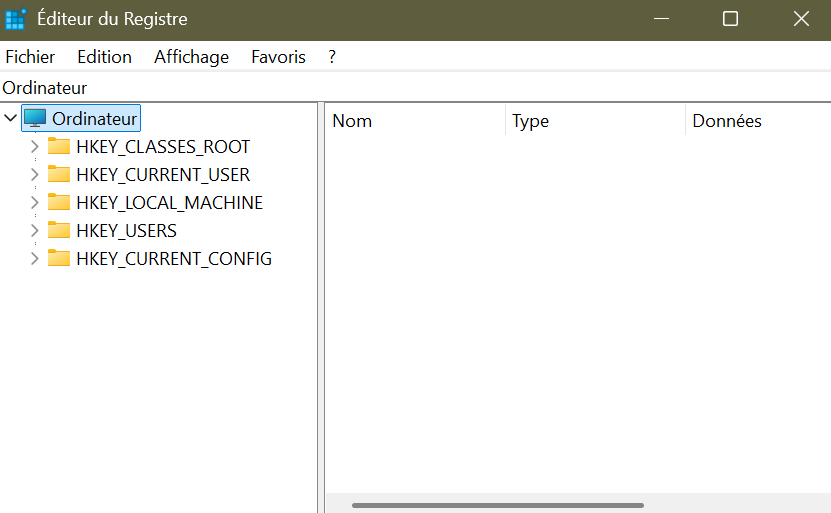
\includegraphics{contents/img/editeur_registre.png}
\end{center}

\vspace{0.5cm}

\noindent Les paramètres généraux de Windows Update sont dans :

\begin{center}
  \begin{verbatim}
    HKLM\SOFTWARE\Microsoft\WindowsUpdate\UX\Settings4
  \end{verbatim}
\end{center}

\noindent Vous y retrouvez les paramètres que l’on peut fixer via l’interface graphique.

\vspace{0.5cm}

14. Sous Windows 2022 server : quel est le rôle qui permet de dédier des serveurs à la gestion et au stockage des mises à jours ? Vous pouvez explorer les rôles possibles de votre VM serveur Windows 2022 et le trouver facilement. Quelle commande PowerShell permet de lister les rôles du serveur ?

\begin{center}
  \begin{verbatim}
    # Le rôle est "Windows Server Update Services (WSUS)".
    # La commande PowerShell pour lister les rôles du serveur est :
    Get-WindowsFeature
  \end{verbatim}
\end{center}

\vspace{0.5cm}

15. Vous devez vérifier les mises à jours sur votre VM Ubuntu Server, les installer si c’est nécessaire et
programmer une mise à jour régulière.
Comment vérifier s’il existe des mises à jour ? Comment les installer ? Comment les programmer ?

\begin{verbatim}
# Pour vérifier les mises à jour sur Ubuntu Server :
sudo apt update

# Pour installer les mises à jour disponibles :
sudo apt upgrade -y

# Pour programmer une mise à jour régulière, vous pouvez utiliser cron.
# Par exemple, pour exécuter une mise à jour quotidienne à 2h du matin,
# ajoutez la ligne suivante au crontab avec 'crontab -e' :
0 2 * * * sudo apt update && sudo apt upgrade -y
\end{verbatim}

\subsection*{Paramétrage de Windows}
\phantomsection
\addcontentsline{toc}{subsection}{Paramétrage de Windows}
\noindent La stratégie de sécurité locale de Windows permet de configurer de nombreux éléments de sécurité pour un ordinateur particulier. . Quand les PC font partie d'un domaine Active Directory vous pourrez utiliser les stratégies de groupe au niveau du domaine.

\vspace{0.5cm}

16. Comment modifier les stratégies de sécurité locales d'un poste particulier ? Quel droit faut il ?

\begin{center}
  \begin{verbatim}
  # Pour modifier les stratégies de sécurité locales d'un poste,
  # ouvrez l'éditeur de stratégie de sécurité locale en exécutant
  # "secpol.msc" depuis la boîte de dialogue Exécuter (Win + R).
  # Vous devez avoir des droits d'administrateur pour effectuer
  # ces modifications.
  \end{verbatim}
\end{center}

\subsection*{Excercices d'application}
\phantomsection
\addcontentsline{toc}{subsection}{Excercices d'application}
\noindent Créez un compte \textbf{Administrateur local protégé par mot de passe} sur le poste de travail (seul compte
autorisé à exécuter des tâches d’administration sur le poste).
Créez un compte \textbf{utilisateur local} membre du groupe local \textbf{"Utilisateurs"}.
Pour cet exercice, \textbf{l’administrateur} du poste de travail s’appellera \textbf{"Admin"}, et l’utilisateur s’appellera
\textbf{"Utilisateur1"}. N’oubliez pas de les remplacer à chaque fois par des noms d’utilisateurs qui sont propres
à votre environnement

\begin{center}
  \begin{verbatim}
    # Créer le compte Administrateur local
    $adminUsername = "Admin"
    $adminPassword = Read-Host "Entrez le mot de passe pour
    l'administrateur" -AsSecureString
    New-LocalUser -Name $adminUsername 
      -Password $adminPassword 
      -FullName "Administrateur Local" 
      -Description "Compte administrateur local"
    Add-LocalGroupMember -Group "Administrators" -Member $adminUsername
    Write-Host "Le compte administrateur local '$adminUsername' a été
    créé avec succès."
    # Créer le compte utilisateur local
    $userUsername = "Utilisateur1"
    $userPassword = Read-Host "Entrez le mot de passe pour
    l'utilisateur" -AsSecureString
    New-LocalUser -Name $userUsername 
      -Password $userPassword 
      -FullName "Utilisateur Local" 
      -Description "Compte utilisateur local"
    Add-LocalGroupMember -Group "Users" -Member $userUsername
    Write-Host "Le compte utilisateur local '$userUsername' a été
    créé avec succès."
  \end{verbatim}
\end{center}

\vspace{0.5cm}

17. Comment créer une stratégie de securité locale qui bloque le port USB d'un PC physique quand un utilisateur particulier, Utilisateur1, se connecte ? Pourquoi le faire ?

\begin{center}
  \begin{verbatim}
    # Pour créer une stratégie de sécurité locale qui bloque
    # le port USB
    # pour un utilisateur spécifique, vous pouvez utiliser l'éditeur
    # de stratégie
    # de sécurité locale (secpol.msc) et configurer les paramètres
    # de restriction
    # des périphériques amovibles.
    # Cependant, cette fonctionnalité n'est pas directement disponible
    # pour un utilisateur spécifique via secpol.msc. Vous devrez utiliser
    # des stratégies de groupe (GPO) dans un environnement Active
    # Directory pour appliquer cette restriction à un utilisateur
    # spécifique.
    #
    # Le blocage des ports USB peut être fait pour des raisons de
    # sécurité, afin d'empêcher l'introduction de logiciels
    # malveillants via des périphériques
    # USB ou pour protéger les données sensibles contre le vol.
  \end{verbatim}
\end{center}

18. Comment mettre en place une stratégie de mot de passe locale sur un poste et pourquoi ?

\begin{center}
  \begin{verbatim}
    # Pour mettre en place une stratégie de mot de passe locale,
    # ouvrez l'éditeur de stratégie de sécurité locale en exécutant
    # "secpol.msc" depuis la boîte de dialogue Exécuter (Win + R).
    # Naviguez vers "Stratégies de compte" > "Stratégie de mot de passe".
    # Vous pouvez définir des paramètres tels que la
    # longueur minimale du mot de passe,
    # la complexité requise, et la durée de vie maximale du mot de passe.
    #
    # Mettre en place une stratégie de mot de passe est important pour
    # renforcer la sécurité des comptes utilisateurs, réduire le risque
    # d'accès non autorisé et protéger les données sensibles.
  \end{verbatim}
\end{center}

\vspace{0.5cm}

19. Comment activer le contrôle des applications (AppLocker) ? Pourquoi l'activer ?

\begin{center}
  \begin{verbatim}
    # Pour activer AppLocker, ouvrez l'éditeur de stratégie de
    # sécurité locale en exécutant "secpol.msc" depuis la boîte
    # de dialogue Exécuter (Win + R).
    # Naviguez vers "Stratégies de contrôle des 
    # applications" > "AppLocker".
    # Vous pouvez créer des règles pour les exécutables, les scripts,
    # les fichiers DLL, etc., afin de contrôler quelles
    # applications peuvents'exécuter sur le système.
    #
    # Activer AppLocker est important pour renforcer la sécurité en
    # empêchant l'exécution de logiciels non autorisés ou malveillants,
    # ce qui aide à protéger le système contre les attaques et les
    # infections par des logiciels malveillants.
  \end{verbatim}
\end{center}

\subsection*{Paramétrage des mises à jours Windows}
\phantomsection
\addcontentsline{toc}{subsection}{Paramétrage des mises à jours Windows}
\noindent Une stratégie de groupe locale (ou Local Group Policy) est un ensemble de paramètres de configuration qui s'appliquent à un ordinateur Windows de manière locale, c'est-à-dire sans nécessiter de connexion à un réseau ou à un serveur Active Directory (AD).
Connectez vous avec le compte administrateur : 
\begin{itemize}
  \item Appuyez sur les touches Windows + R pour ouvrir la fenêtre Exécuter
  \item Tapez gpedit.msc et appuyez sur Entrée
\end{itemize}

\vspace{0.5cm}

20. Comment utiliser une stratégies de groupe locale pour paramétrer Windows update et Windows defender ?

\begin{center}
  \begin{verbatim}
    # Pour paramétrer Windows Update via la stratégie de groupe locale,
    # ouvrez l'éditeur de stratégie de groupe locale (gpedit.msc).
    # Naviguez vers "Configuration ordinateur" >
    # "Modèles d'administration"
    # > "Composants Windows" > "Windows Update".
    # Vous pouvez configurer des paramètres tels que la planification
    # des mises à jour automatiques, les notifications, et plus encore.
    
    
    
    
    
    # Pour paramétrer Windows Defender, naviguez vers
    # "Configuration ordinateur" > "Modèles d'administration"
    # > "Composants Windows" > "Microsoft Defender Antivirus".
    # Vous pouvez configurer des paramètres tels que la protection en
    # temps réel, les exclusions, et d'autres options de sécurité.
  \end{verbatim}
\end{center}

\subsection*{Les systèmes Linux ne sont pas à l'abri des ransomwares}
\phantomsection
\addcontentsline{toc}{subsection}{Les systèmes Linux ne sont pas à l'abri des ransomwares}
\noindent Les attaques de ransomware sur les réseaux Linux sont menées par des moyens plus subversifs que les
attaques sur un système Windows. Les acteurs malveillants recherchent les vulnérabilités des
composants des systèmes Linux.

\noindent Les machines virtuelles, les conteneurs et les services de stockage en nuage fonctionnant sous Linux
sont souvent pris pour cible, surtout s'ils ne disposent pas de contrôles d'accès appropriés.
De nombreux sites web et services en ligne fonctionnent sous Linux. Les ransomwares peuvent se
propager par le biais de plateformes CMS compromises, de plugins obsolètes ou d'identifiants
d'administration faibles.

\noindent  Les périphériques NAS fonctionnent souvent avec un système d'exploitation basé sur Linux et stockent
des sauvegardes critiques, ce qui en fait des cibles précieuses.
Au-delà des serveurs traditionnels et de l'infrastructure en nuage, un nombre croissant de dispositifs IoT
basés sur Linux sont également des cibles potentielles.
Si tout système Linux vulnérable peut être la cible d'un ransomware, certains types d'appareils
présentent un risque plus élevé en raison de leur fonction et de leurs faiblesses communes en matière
de sécurité :
\noindent Les entreprises qui utilisent des serveurs basés sur Linux pour les bases de données, les applications et
le stockage sont des cibles de choix. Les attaquants exploitent les faiblesses de SSH, les logiciels non
corrigés et les mauvaises configurations.

\noindent Pour les prévenir, il est important de savoir maintenir les logiciels à jour, de savoir restreindre les
privilèges, de savoir mettre une politique de mots de passe forts et de savoir restreindre la sécurité SSH.

\subsection*{GESTION DES UTILISATEUR AVEC UBUNTU SERVER}
\phantomsection
\addcontentsline{toc}{subsection}{GESTION DES UTILISATEUR AVEC UBUNTU SERVER}
\noindent La gestion des utilisateurs est une partie cruciale de la sécurisation du système. Une gestion inefficace des utilisateurs et de leurs droits conduit souvent de nombreux systèmes a être corrompus. Il est donc fondamental de comprendre comment vous pouvez protéger votre serveur aux travers de techniques simples de gestion des comptes utilisateurs.

\newpage 

21. Comment gérer les utilisateurs et les groupes ?

\begin{center}
  \begin{verbatim}
  # Pour gérer les utilisateurs sur Ubuntu Server, vous pouvez utiliser
  # les commandes suivantes :
  #
  # Ajouter un nouvel utilisateur :
  sudo adduser nom_utilisateur
  #
  # Supprimer un utilisateur :
  sudo deluser nom_utilisateur
  #
  # Ajouter un utilisateur à un groupe :
  sudo usermod -aG nom_groupe nom_utilisateur
  #
  # Supprimer un utilisateur d'un groupe :
  sudo gpasswd -d nom_utilisateur nom_groupe
  #
  # Lister les utilisateurs :
  cut -d: -f1 /etc/passwd
  #
  # Lister les groupes :
  cut -d: -f1 /etc/group
  \end{verbatim}
\end{center}

\vspace{0.5cm}

22. Comment gérer la politique des mots de passe sur un serveur Ubuntu?

\begin{center}
  \begin{verbatim}
  # Pour gérer la politique des mots de passe sur Ubuntu Server,
  # vous pouvez modifier le fichier /etc/pam.d/common-password
  # et utiliser le module pam_pwquality.so pour définir des règles
  # de complexité des mots de passe.
  #
  # Par exemple, pour exiger une longueur minimale de mot de passe
  # et des caractères spéciaux, vous pouvez ajouter ou modifier
  # la ligne suivante dans /etc/pam.d/common-password :
  password requisite pam_pwquality.so retry=3 minlen=12 ucredit=-1
  lcredit=-1 dcredit=-1 ocredit=-1
  #
  # Après avoir modifié le fichier, enregistrez les changements
  # et les nouvelles politiques seront appliquées lors de la
  # création ou du changement de mot de passe.
  \end{verbatim}
\end{center}

\newpage

23. Comment restreindre l'accès en SSH aux seuls comptes utilisateurs qui devrait l'avoir ?

\begin{center}
  \begin{verbatim}
  # Pour restreindre l'accès SSH aux seuls comptes utilisateurs
  # autorisés, vous pouvez modifier le fichier de configuration
  # SSH situé à /etc/ssh/sshd_config.
  #
  # Ajoutez la ligne suivante pour spécifier les utilisateurs
  # autorisés à se connecter via SSH :
  AllowUsers utilisateur1 utilisateur2
  #
  # Vous pouvez également utiliser AllowGroups pour autoriser
  # uniquement les membres d'un groupe spécifique :
  AllowGroups groupe_ssh
  #
  # Après avoir modifié le fichier, enregistrez les changements
  # et redémarrez le service SSH pour appliquer les modifications :
  sudo systemctl restart sshd
  \end{verbatim}
\end{center}


24. Comment maintenir son serveur et ses logiciels à jour ?

\begin{center}
  \begin{verbatim}
  # Pour maintenir votre serveur Ubuntu et ses logiciels à jour,
  # vous pouvez utiliser les commandes suivantes :
  #
  # Mettre à jour la liste des paquets disponibles :
  sudo apt update
  #
  # Mettre à niveau les paquets installés vers leurs
  # dernières versions :
  sudo apt upgrade
  #
  # Pour une mise à niveau complète, incluant les
  # changements de dépendances :
  sudo apt full-upgrade
  #
  # Nettoyer les paquets obsolètes :
  sudo apt autoremove
  \end{verbatim}
\end{center}

\newpage


\section*{Analyse et résolution : La rançon du Cyberespace}
\addcontentsline{toc}{section}{Analyse et résolution : La rançon du Cyberespace}

\noindent\textbf{Rappel des commandes PowerShell et Bash utilisées}

\noindent\textbf{Windows — PowerShell}

\begin{lstlisting}[language=bash]
# Verifier l'etat du pare-feu
Get-NetFirewallProfile

# Activer le pare-feu sur tous les profils
Set-NetFirewallProfile -Profile Domain,Public,Private -Enabled True

# Lister les mises a jour disponibles
Get-WindowsUpdate

# Installer toutes les mises a jour
Install-WindowsUpdate -AcceptAll -AutoReboot

# Desactiver les services inutiles
Set-Service -Name "Spooler" -StartupType Disabled

# Verifier les comptes locaux
Get-LocalUser

# Activer l'audit avance
auditpol /set /category:* /success:enable /failure:enable

# Lister les ports ouverts
Get-NetTCPConnection

# Activer la protection Windows Defender
Set-MpPreference -DisableRealtimeMonitoring $false
\end{lstlisting}

\vspace{1cm}

\noindent\textbf{Ubuntu — Bash}

\begin{lstlisting}[language=bash]
# Mise a jour du système
sudo apt update && sudo apt upgrade -y

# Verifier les services actifs
systemctl list-units --type=service

# Desactiver un service inutile
sudo systemctl disable bluetooth.service --now

# Configurer UFW
sudo ufw enable
sudo ufw default deny incoming
sudo ufw default allow outgoing

# Lister les ports ouverts
sudo ss -tulnp

# Verifier les comptes et groupes
cat /etc/passwd
cat /etc/group

# Installer les outils de securite essentiels
sudo apt install fail2ban unattended-upgrades -y

# Activer les mises a jour automatiques
sudo dpkg-reconfigure unattended-upgrades

# Verifier l'integrite du système
sudo debsums -s
\end{lstlisting}

\vspace{1cm}

\noindent Réalisation d'une brochure de sensibilisation aux risques liés aux ransomwares à destination des utilisateurs finaux.

\vspace{1cm}

\begin{center}
    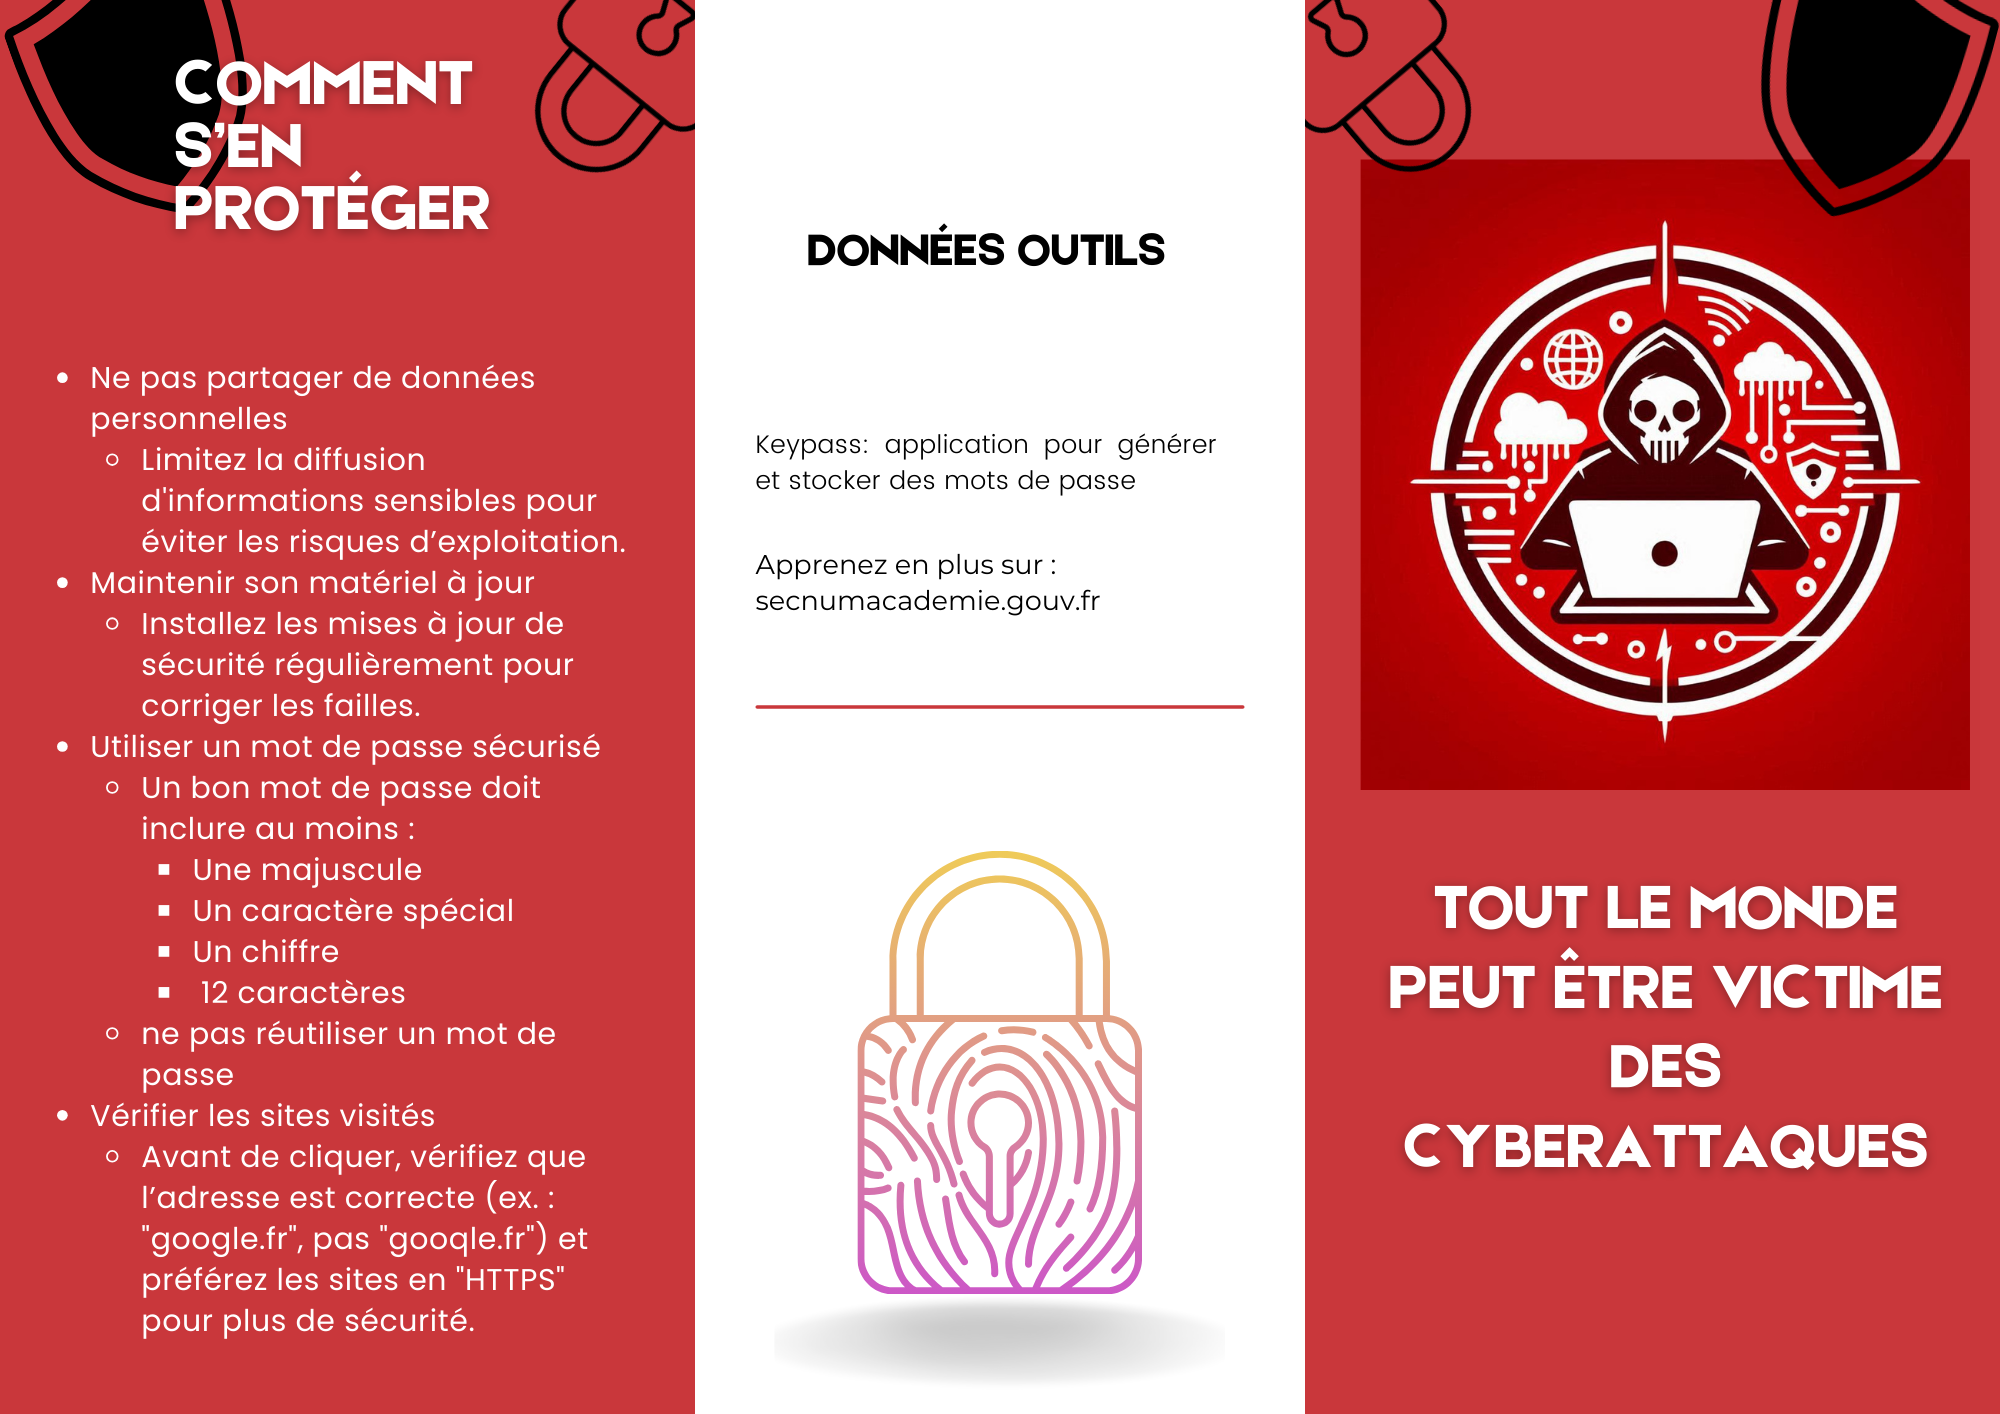
\includegraphics[width=1\textwidth]{contents/img/brochure_1.png}

    \vspace{1cm}

    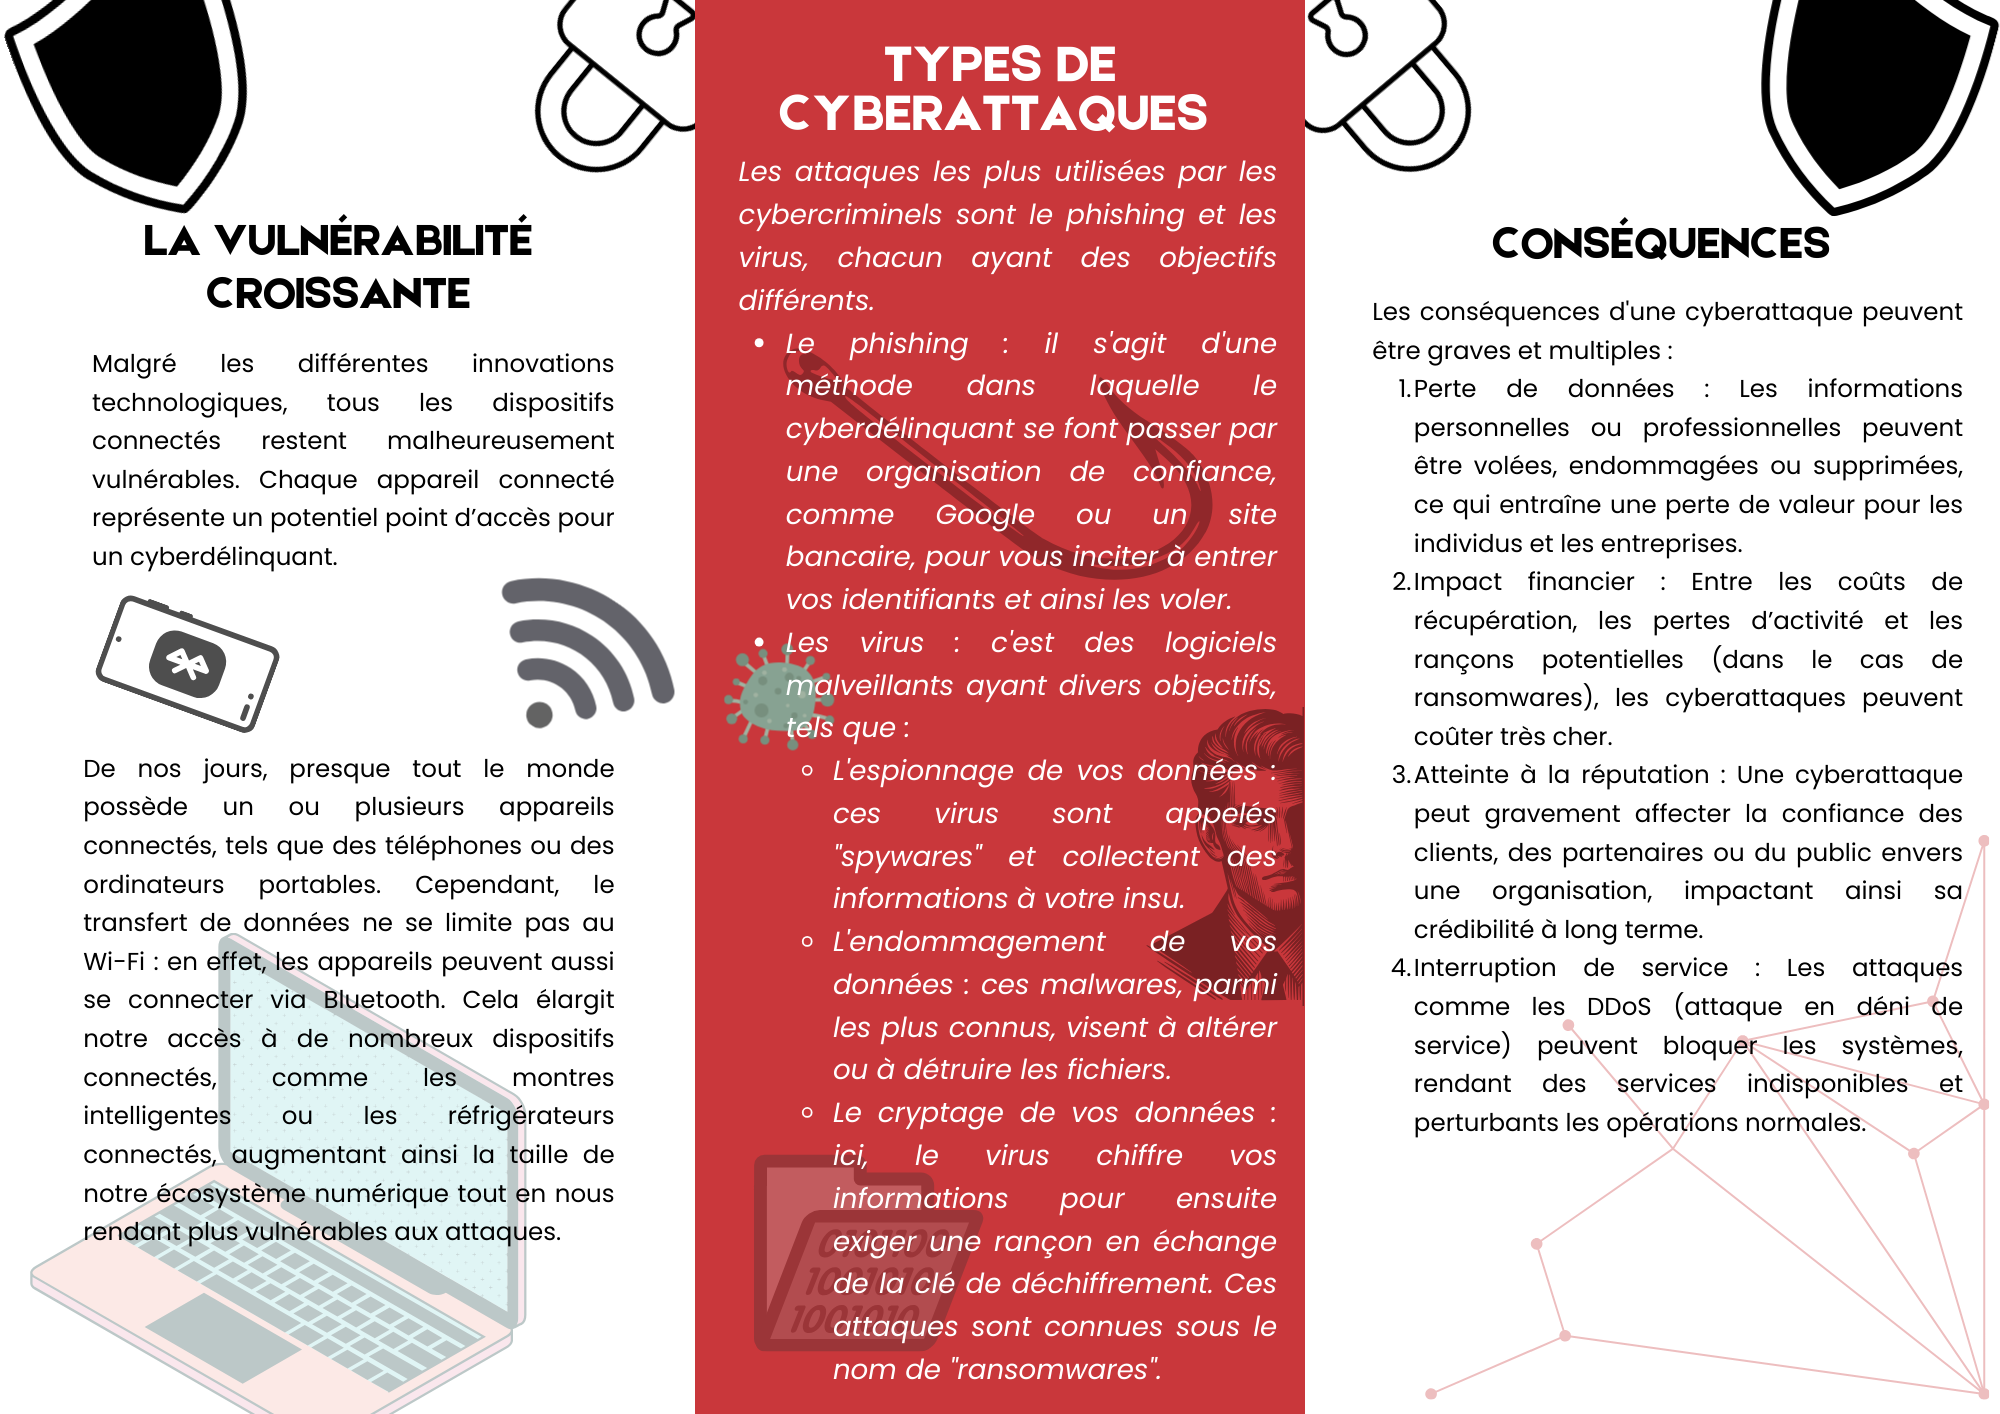
\includegraphics[width=1\textwidth]{contents/img/brochure_2.png}
\end{center}


\section*{Conclusion}
\addcontentsline{toc}{section}{Conclusion}
Ce document a permis de revoir les notions de base de PowerShell, la gestion des utilisateurs locaux sur un poste Windows, la sécurité des postes Windows avec Windows Security, la protection antivirus, la mise à jour des systèmes d'exploitation Windows et Ubuntu Server, la navigation et la modification du registre Windows, le paramétrage de Windows via les stratégies de groupe locales, ainsi que la gestion des utilisateurs et la sécurité sur Ubuntu Server.

\newpage

\section*{Capitalisation}
\addcontentsline{toc}{section}{Capitalisation}
\noindent Ce document a permis de revoir les notions suivantes :
\begin{itemize}
  \item Les bases de PowerShell et la création de scripts simples.
  \item La gestion des utilisateurs locaux sur un poste Windows.
  \item La sécurité des postes Windows avec Windows Security.
  \item La protection antivirus et l'utilisation du fichier de test Eicar.
  \item La mise à jour des systèmes d'exploitation Windows et Ubuntu Server.
  \item La navigation et la modification du registre Windows.
  \item Le paramétrage de Windows via les stratégies de groupe locales.
  \item La gestion des utilisateurs et la sécurité sur Ubuntu Server.
\end{itemize}

\section*{Ressources}
\addcontentsline{toc}{section}{Ressources}
\begin{itemize}
  \item Corbeille d'Excercice.
  \item Documentation officielle de PowerShell : 
    \url{https://docs.microsoft.com/fr-fr/powershell/}
  \item Documentation officielle d'Ubuntu Server :
    \url{https://ubuntu.com/server/docs}
  \item Tutoriels sur la gestion des utilisateurs et la sécurité sous Linux :
    \url{https://linuxconfig.org/}
  \item Tutoriels sur la gestion des utilisateurs et la sécurité sous Windows :
\end{itemize}